\begin{mainquestion}{bridgefilter}{Bridge-Circuit RC Filter}

Consider the bridge circuit shown on the right.

\begin{center}
    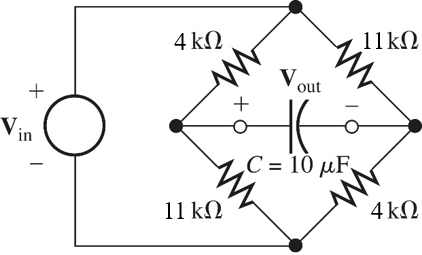
\includegraphics[width=4.3in]{bridge_circuit.png}
\end{center}

\begin{partquestion}{transferfunction}{Find the transfer function $H\left(j\omega\right) = \frac{\mathbf{V_{\text{out}}}}{\mathbf{V_{\text{in}}}}$ of the circuit. \textit{Hint: Find a Th\'evenin equivalent for the circuit seen by the capacitor.}}
\begin{answer}
To find the Th\'evenin resistance, we short the voltage source and look into the circuit from the perspective of the capacitor. With the voltage shorted, the potential at the top node of the circuit is the same as that of the bottom node---they are thus the same node. So the resistance is just:
\begin{align*}
R_{\mathrm{th}}&=\left(\qty{4}{\kilo\ohm}||\qty{11}{\kilo\ohm}\right)+\left(\qty{4}{\kilo\ohm}||\qty{11}{\kilo\ohm}\right)\\
&=2\frac{(4)(11)}{4+11}\\
&=\frac{88}{15} \qty{ }{\kilo\ohm}
\end{align*}

To find the Thevenin (open-circuit) voltage, we remove the capacitor and notice that it will be just the difference between two voltage dividers:
\begin{align*}
\mathbf{V_{th}} &= \frac{11}{4+11}\mathbf{V_{in}}- \frac{4}{4+11}\mathbf{V_{in}}\\
&=\frac{7}{15}\mathbf{V_{in}}
\end{align*}


We can write the equivalent circuit as follows:

\begin{center}
    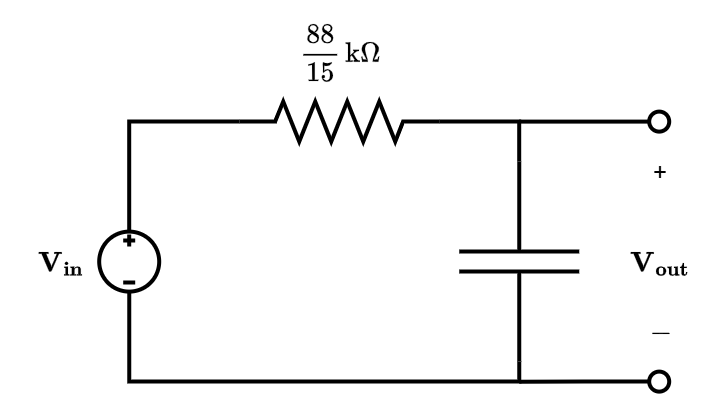
\includegraphics[width=4.8in]{thevenin_equivalent.png}
\end{center}

From here, we can directly write the transfer function as a voltage divider with complex impedances:
\begin{align*}
H\left(j\omega\right) &= \frac{\mathbf{V_{\text{out}}}}{\mathbf{V_{\text{in}}}}\\
&=\left(\frac{7}{15}\right)\frac{\frac{1}{j\omega C}}{(R+\frac{1}{j\omega C}}\\
&=\frac{\frac{7}{15}}{1+j\omega RC}\\
&=\frac{\frac{7}{15}}{1+j\omega\left(\frac{88}{15}\times10^3\right)\left(10\times10^{-6}\right)}\\
&=\frac{\frac{7}{15}}{1+j\omega\left(\frac{22}{375}\right)}\\
&=\frac{175}{375+j22\omega}
\end{align*}
\end{answer}
\end{partquestion}

\begin{partquestion}{functionality}{Based on the result from (a), identify the functionality of this circuit (what does it do?)}
\begin{answer}
This is a low pass filter.
\end{answer}
\end{partquestion}

\begin{partquestion}{bodesketch}{Plot a sketch (to scale) of $\left|H\left(j\omega\right)\right|$ and $\angle H\left(j\omega\right)$.}
\begin{answer}
The magnitude is:

\begin{center}
    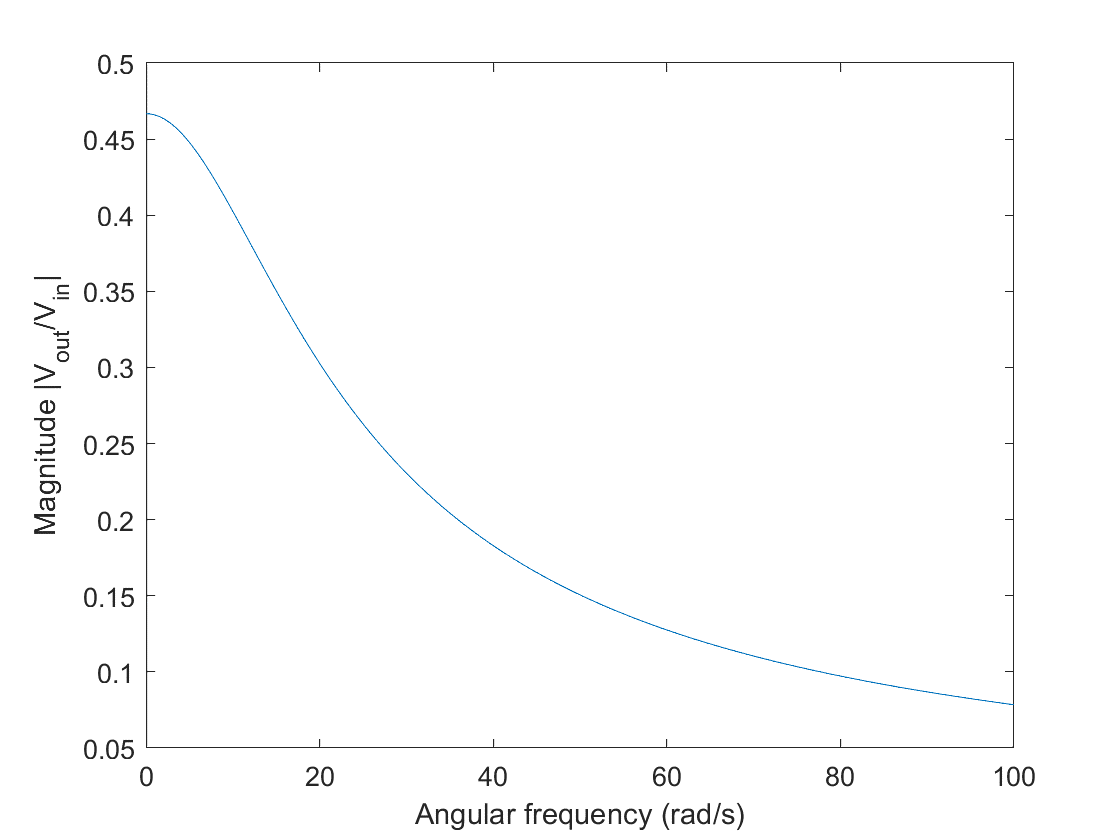
\includegraphics[width=5.3in]{magnitude_plot.png}
\end{center}

The phase is:

\begin{center}
    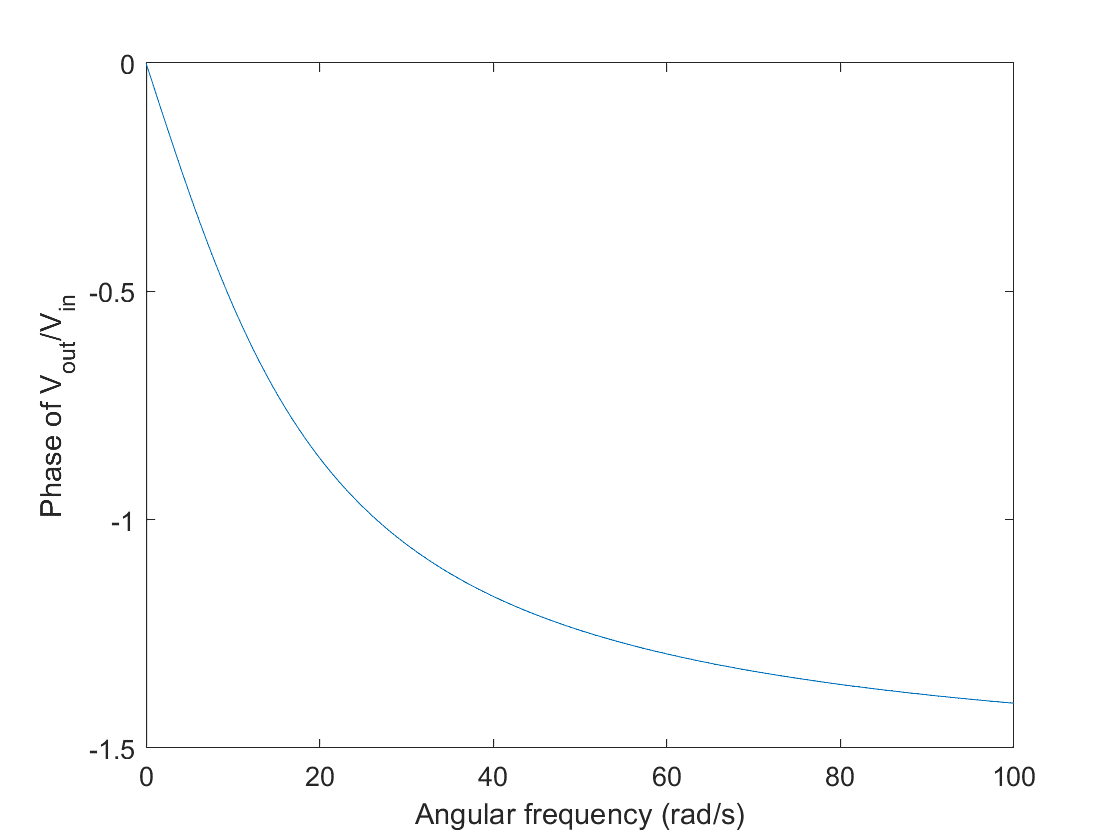
\includegraphics[width=5.3in]{phase_plot.png}
\end{center}
\end{answer}
\end{partquestion}

\begin{partquestion}{cornerfrequency}{What is the corner frequency $\omega_{c}$?}
\begin{answer}
% NOTE: The imported source appears numerically inconsistent with the surrounding circuit and plots. Preserved here for manual review.
We can either estimate it from the graph by finding the angular frequency where the magnitude is 0.707 times the peak value, or we can calculate it directly from the expression for the transfer function. Either way, we should get a similar value: $\omega_{c} = \frac{1}{RC} = \frac{1}{5.867 \times 10^{-2}} = \qty{17}{\radian/\second}$
\end{answer}
\end{partquestion}

\begin{partquestion}{outputvoltage}{What is the output voltage if the input voltage is $v_{i}(t) = 2 + 3\sin\left(\omega_{c}t\right) + 4\sin\left(2\omega_{c}t\right)$?}
\begin{answer}
% NOTE: The final imported expression appears to contain OCR inconsistencies. Preserved here for manual review.
We need to determine the gain and phase of the transfer function for three separate frequencies: DC, the corner frequency, and twice the corner frequency. At DC, the gain is $\frac{7}{15}$ and there is no phase shift, so we will see an output of $2\left(\frac{7}{15}\right) = \frac{14}{15}\text{ V}$ from the DC term. At $\omega_{c}$, there is a gain of $\frac{7}{15}\left(\frac{1}{\sqrt{2}}\right) \approx 0.330$ and a phase shift of $-45^{\circ}$, so we will see an output of $3(0.330)\sin\left(\omega_{c}t - 45^{\circ}\right) = 0.990\sin\left(\omega_{c}t - 45^{\circ}\right)\text{ V}$ from the $\omega_{c}$ component of the input. Looking at the graphs at $2\omega_{c}$, there is a gain of about $0.210$ and a phase shift of about $-63.3^{\circ}$, so we will see an output of $4(0.210)\sin\left(2\omega_{c}t - 63.3^{\circ}\right) = 0.839\sin\left(2\omega_{c}t - 63.3^{\circ}\right)\text{ V}$ from the $2\omega_{c}$ component of the input. Putting this all together, we have:

\[
v_{o}(t) = \frac{14}{15} + 0.990\sin\left(\omega_{c}t - 45^{\circ}\right) + 0.839\sin\left(2\omega_{c}t - 63.3^{\circ}\right)\text{ V.}
\]
\end{answer}
\end{partquestion}

\end{mainquestion}